\section*{Supplementary Materials}

\subsection*{S1. Capability Transitions}

Figure~\ref{fig:trajectory_examples} shows start-to-end aggregate CINC transitions for five selected COW conflicts. Each row aggregates participant capability within the first and last observed conflict years, then reports the direction and magnitude of the capability change.

\begin{figure}[H]
\centering
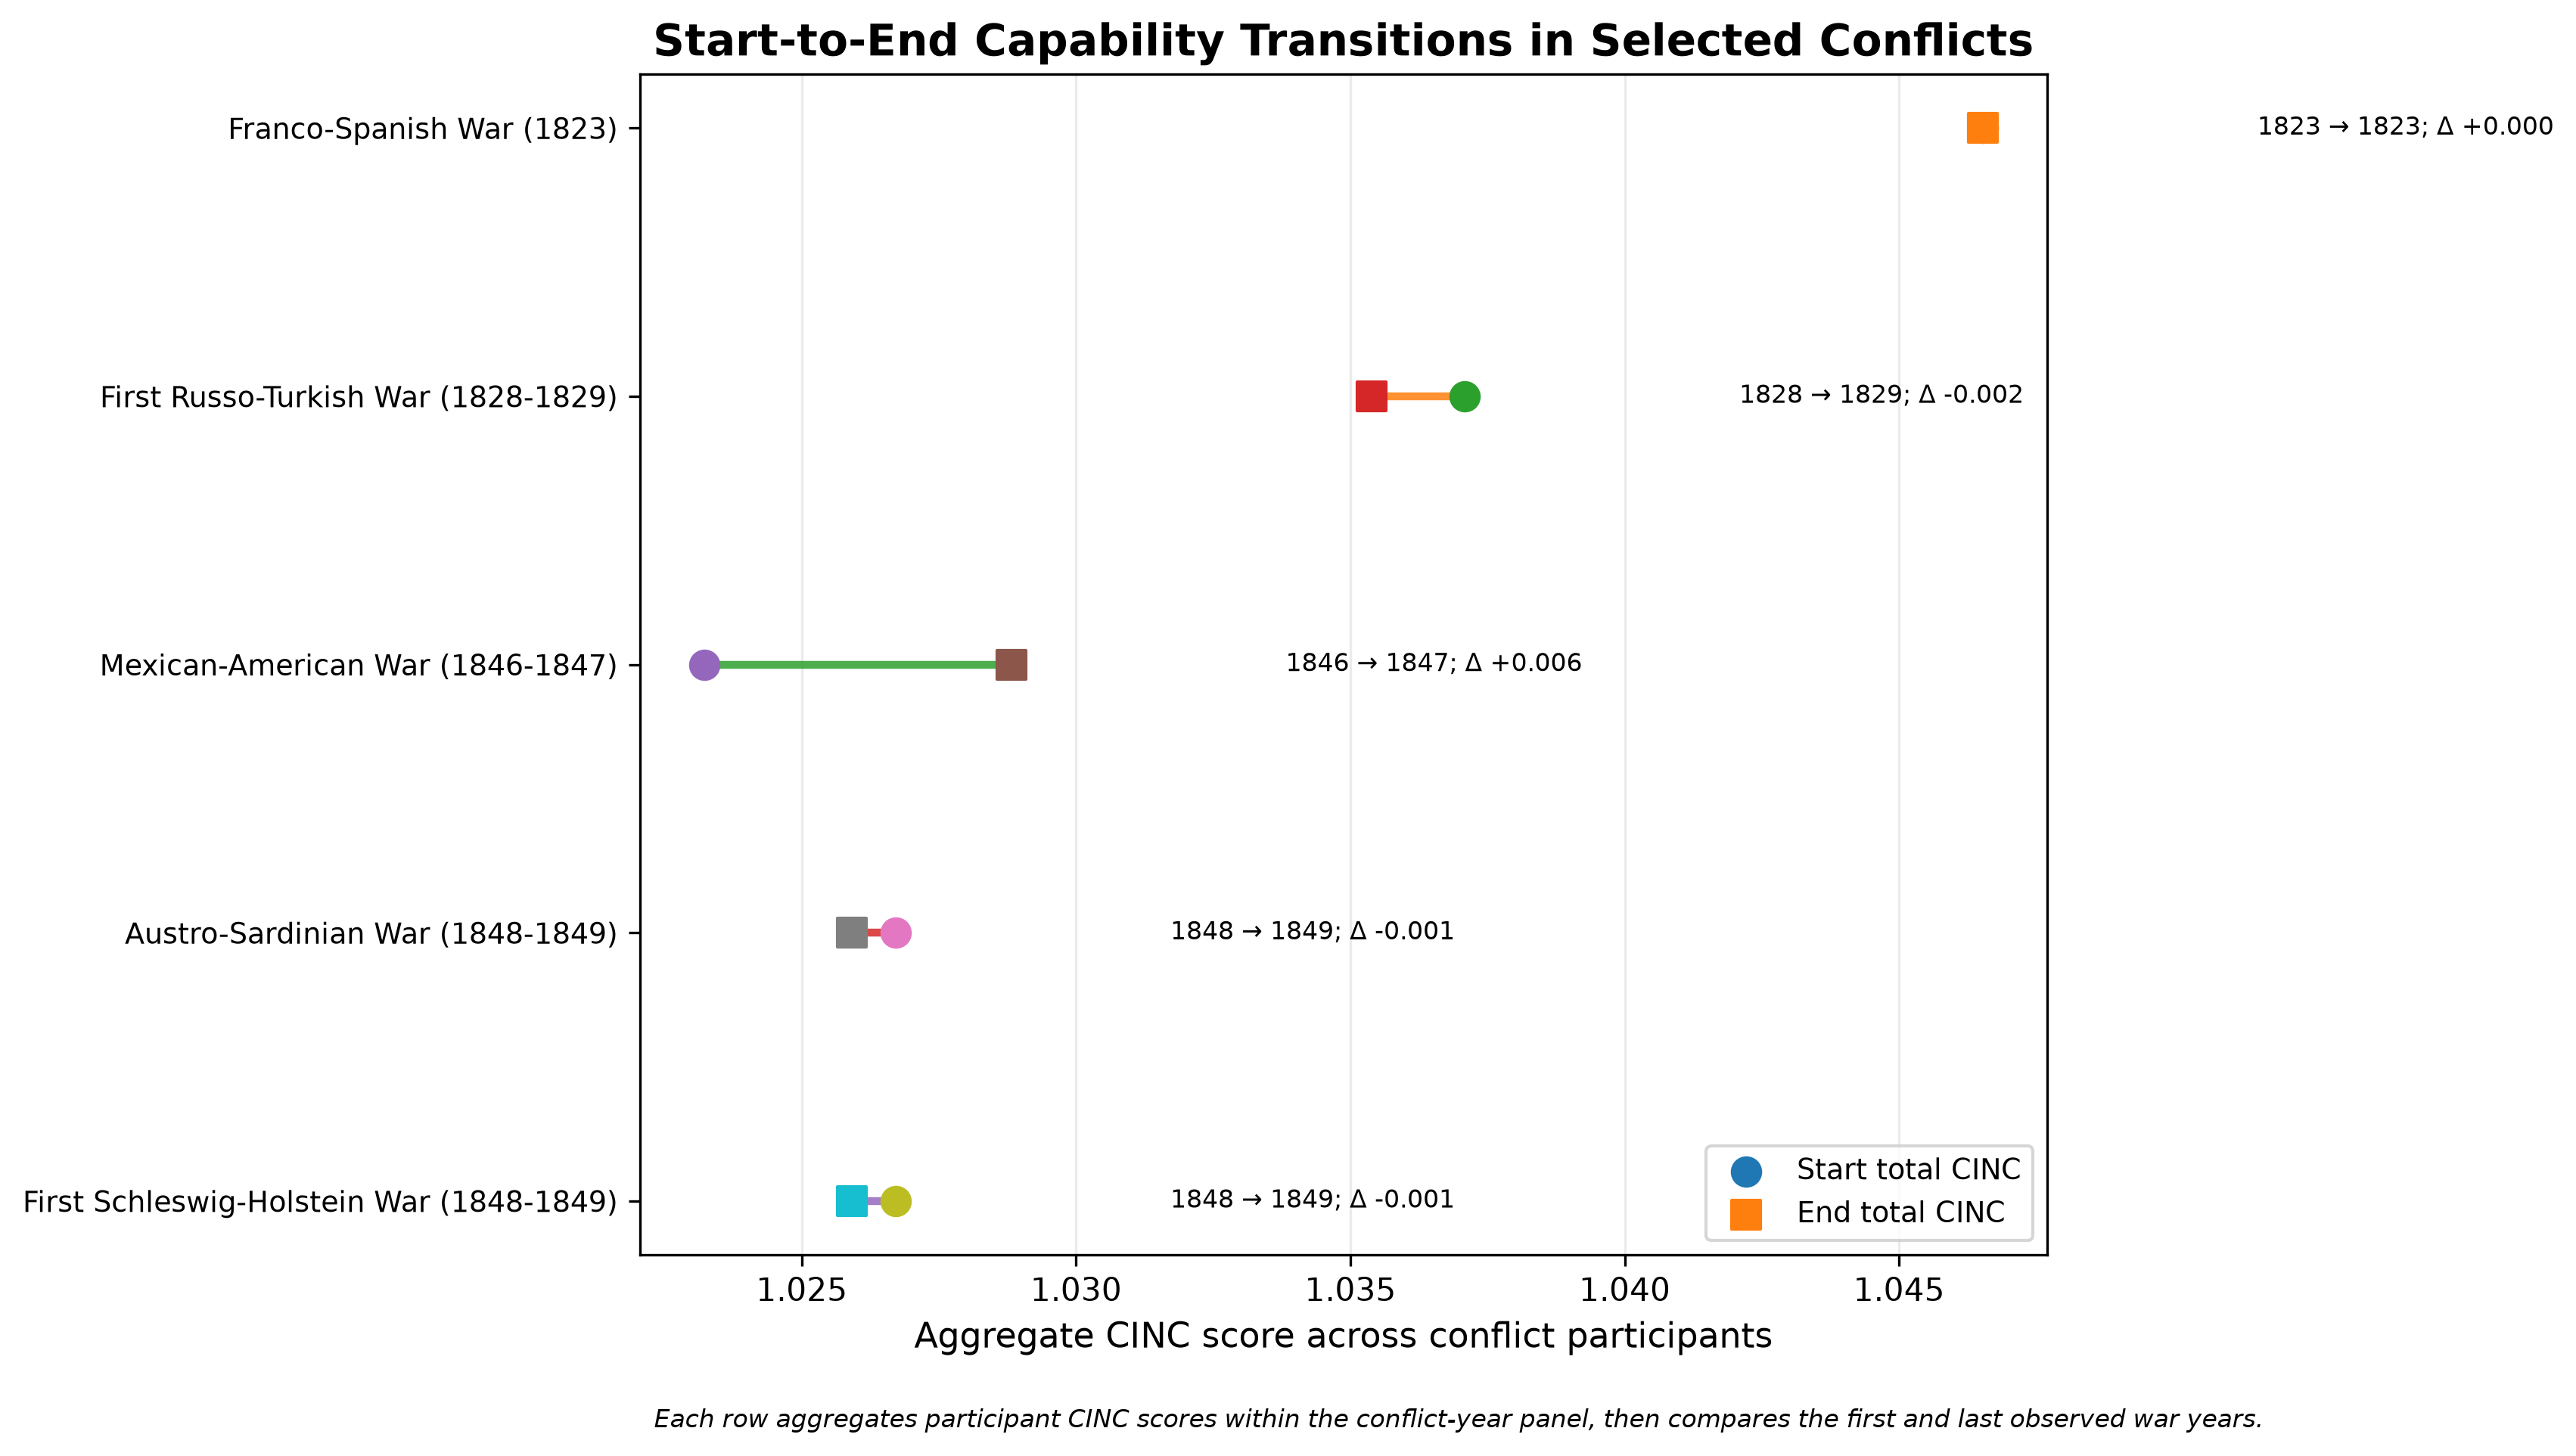
\includegraphics[width=0.65\textwidth]{figures/fig_06_trajectory_examples.png}
\caption{Start-to-end aggregate capability transitions for five selected conflicts. Circles mark the first observed conflict year, squares mark the last observed conflict year, and annotations report the year span and aggregate CINC change.}
\label{fig:trajectory_examples}
\end{figure}

\subsection*{S2. Historical Case Scorecards}

Figure~\ref{fig:case_study_scorecards} presents historical case-study DSS and SES scorecards. The bars show manually assigned historical interpretation scores used for structured comparison; they are not separate model predictions.

\begin{figure}[H]
\centering
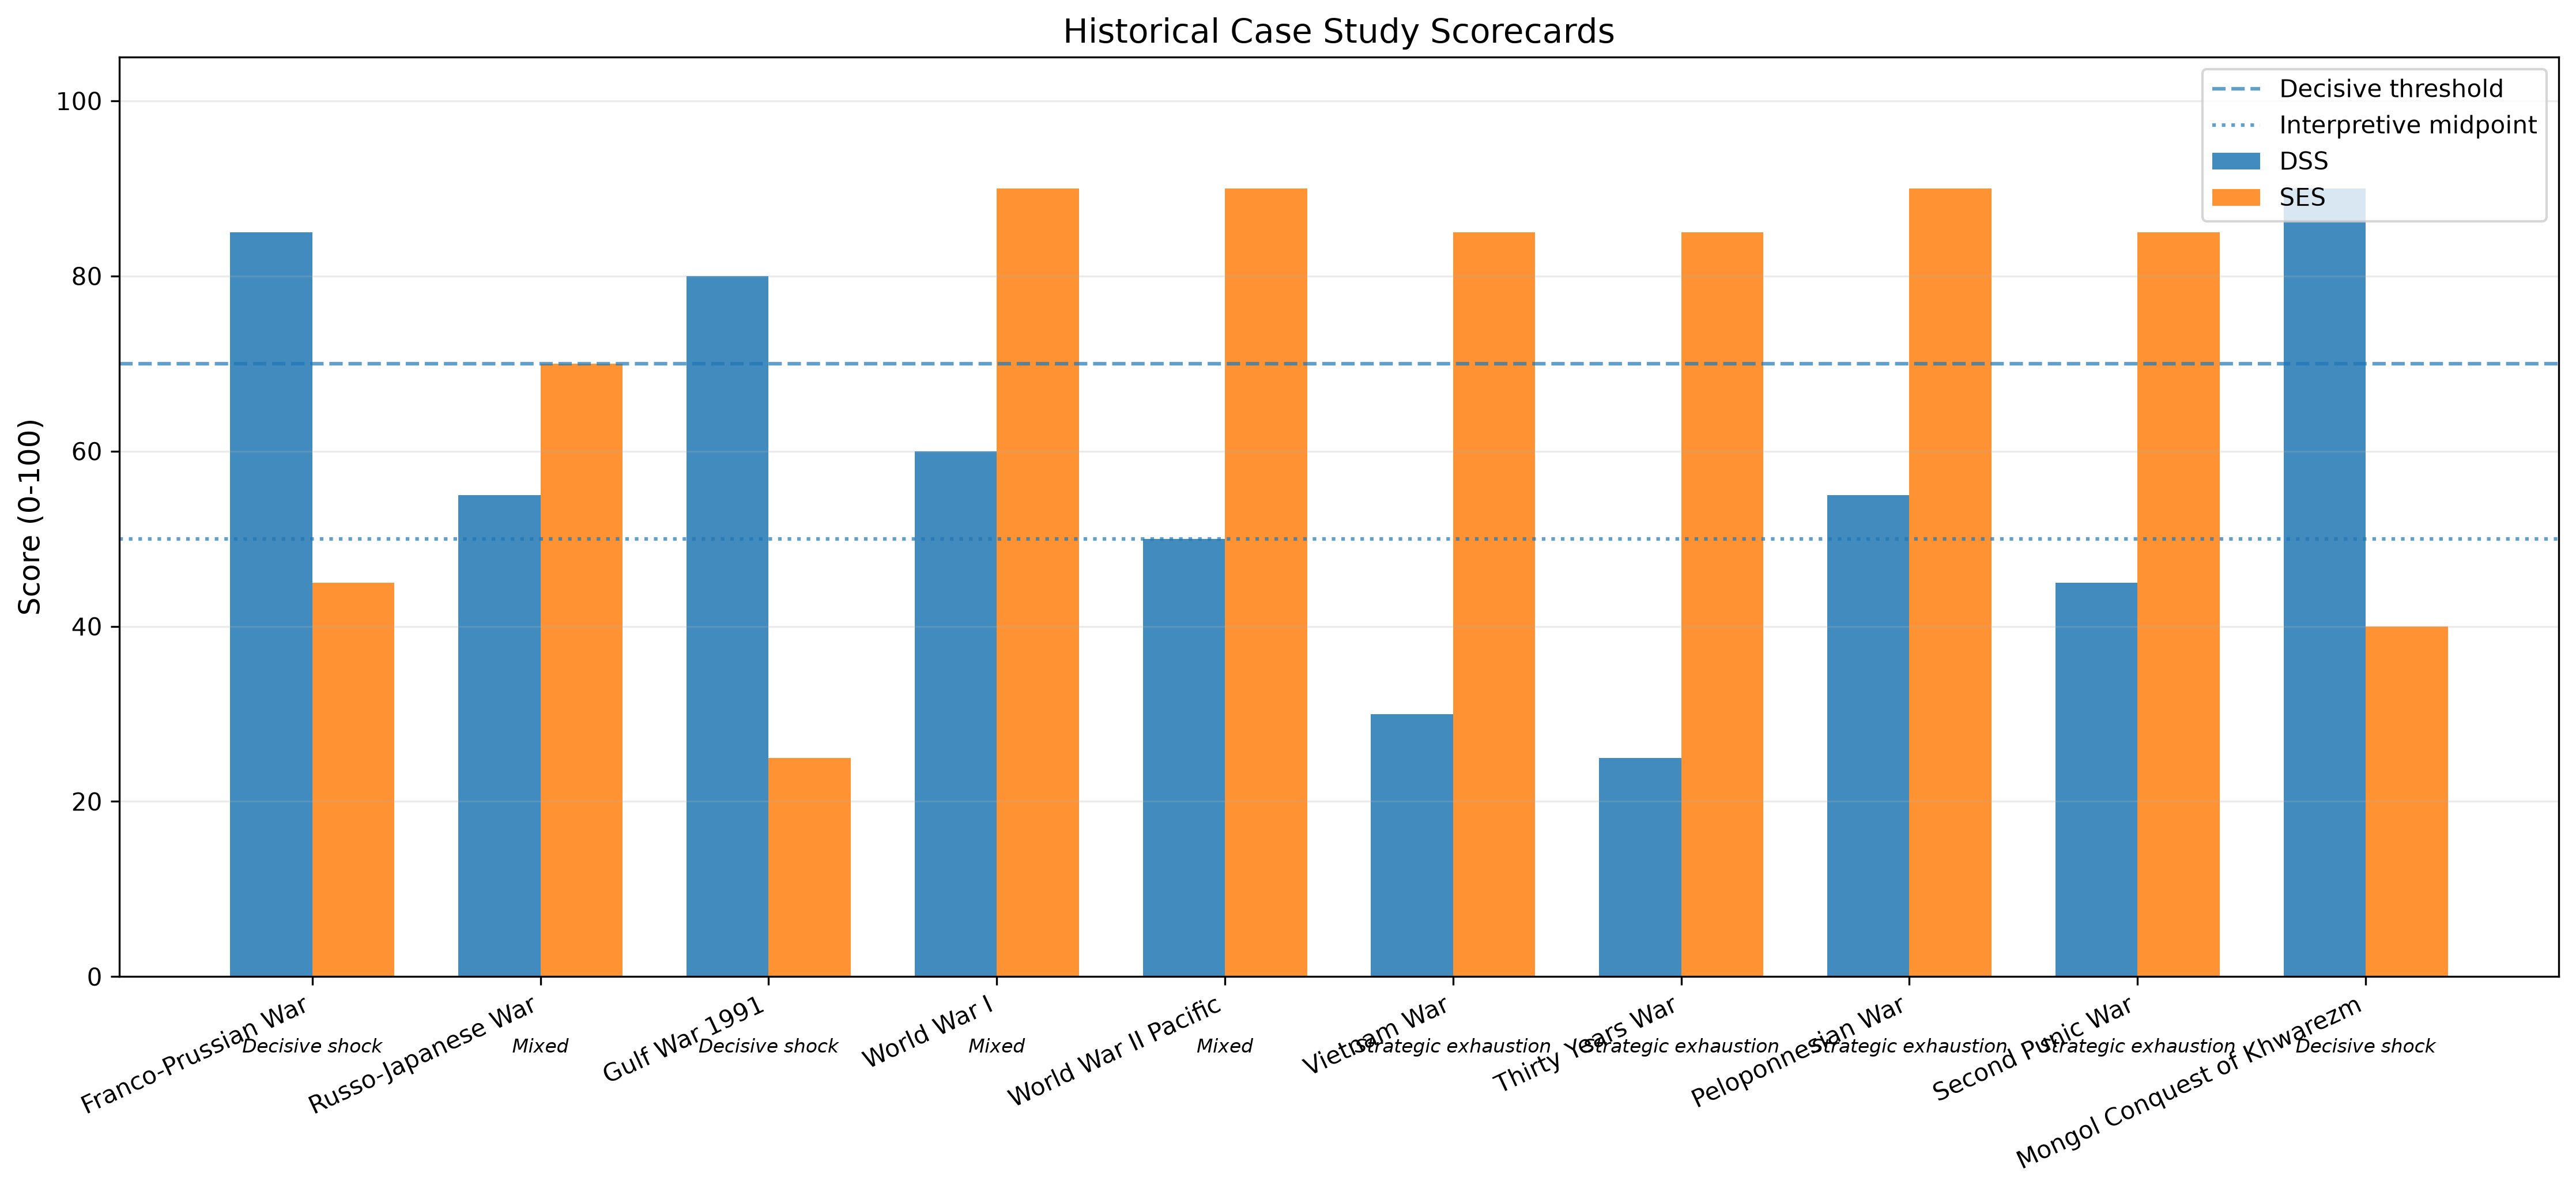
\includegraphics[width=0.65\textwidth]{figures/fig_07_case_study_scorecards.png}
\caption{Historical case-study scorecards. Bars show DSS and SES interpretation scores for selected conflicts.}
\label{fig:case_study_scorecards}
\end{figure}
